\chapter{Mirrors for X-rays}
\label{capitolo2}
\thispagestyle{empty}
\vspace{0.5cm}

\noindent As discussed in Chapter \ref{Introduzione}, to focus X-ray radiation, refraction(compound refractive lenses) and reflection optics (curved mirrors) can be used. In this chapter the reflection optics is discussed because it is the main effect used in my python library. These optics are used in a grazing configuration because with small critical angle for total external reflection for X-ray radiation. The first part of this Chapter discuss as the focusing property of the simplest curved mirror, the spherical one, showing that it can't be used due to its intrinsic aberrations that are huge in a grazing incidence configuration. Then toroidal and conical mirror will be introduced, that cancel out some kind of aberration with respect to the spherical mirror. In the last part the concept of imaging system is discussed. Then  two configurations of conical mirror used to focus the radiation in the synchrotron beamline are explained: the KirckPatrick-Baez system, very popular at ESRF, and the Montel system, that is the main object of my thesis.

\section{Spherical surface}
\noindent Mirrors that carry out any focusing must have a curved surface, is the spherical mirror, the simplest one, that it is defined only by one parameter, the radius of curvature. This mirror works well for normal incidence reflection, but, in a grazing configuration, it is affected by many kinds of aberrations. Here we discussed the:
\begin{enumerate}
\item astigmatism
\item spherical aberration
\end{enumerate}
that are the main aberration that affect the X-ray radiation.
\subsection{Astigmatism}
"Rays that propagate in two perpendicular planes have different foci". This is the definition of astigmatism. In Figure \ref{fig: System1} it is showed the image formation of a beam with a spherical mirror of radius $R $, at grazing incidence $\theta_i $. Supposing that all the rays exiting from the source P are focused in the same point Q, and considering only the part of the beam that hit the portion of the mirror NO, it is possible to define $\beta $ as the source divergence, $\gamma $ the image divergence, $u $ the distance PO and $v $ the distance OQ .
\begin{figure}[]
%
\centering
%
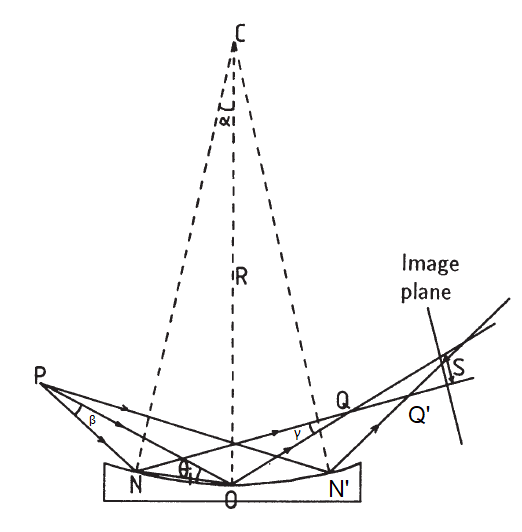
\includegraphics[width=.6\textwidth]{Immagini/Chapter2/System1}
%
\caption{Formation image of a circular mirror for a point-wise source placed at a distance $PO $ from the center of the mirror. $R $ is the curvature of the mirror, $\theta_i $ the angle of the central ray.}
%
\label{fig: System1}
%
\end{figure}
\noindent The beam hit the mirror over a distance equal to $k = $ NO, such as $k<<R $, that correspond to a small divergence $\beta $. The cord NO subtends an angle $\alpha $ with the center of the sphere C, thus $k = R \alpha $, $\gamma $ is the convergence angle of the beam at the focal point Q. For small angle approximation, from the triangle PNO ,
\begin{equation}
\beta = R \alpha \frac{\theta_i - \alpha / 2}{u - R \alpha}
\label{eq: beta}
\end{equation}
\noindent and from QNO
\begin{equation}
\gamma = R \alpha \frac{\theta_i + \alpha / 2}{v + R \alpha}
\label{eq: gamme}
\end{equation}
\noindent The reflection law impose that $\beta + \gamma = 2 \alpha$, thus:
\begin{equation}
\frac{1 - \alpha / (2 \theta_i)}{u - R \alpha} + \frac{1 + \alpha / (2 \theta_i)}{v + R \alpha} = \frac{2}{R \theta_i}
\label{eq: refle lae}
\end{equation}
\noindent in case of paraxial approximation
\begin{equation}
\frac{1}{u} + \frac{1}{v} = \frac{2}{R \theta_i} = \frac{1}{f_m}
\label{eq: reflection law}
\end{equation}
\noindent where
\begin{equation}
f_m = \frac{R \theta_i}{2}
\label{eq: fm}
\end{equation}
\noindent more generally
\begin{equation}
f_m = \frac{R sin \theta_i}{2}
\label{eq: fm2}
\end{equation}
\noindent $f_m $ is named meridian focal length. 
\\
In case of a spherical mirror, a second image is generated in the sagittal plane, as it is showed if Figure \ref{fig: MeridianAndSagittal}, with a focal distance equal to:
\begin{equation}
f_s = \frac{R}{2 \sin \theta_i}
\label{eq: fs}
\end{equation}
\noindent and it is named sagittal focal length.
\begin{figure}[]
%
\centering
%
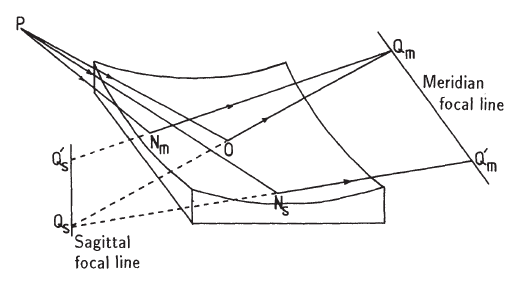
\includegraphics[width=.6\textwidth]{Immagini/Chapter2/MeridianAndSagittal}
%
\caption{Image formation of a spherical mirror. The formation of a point wise source correspond to a two rods, one in the sagittal plane, and the second one in the meridian plane}
%
\label{fig: MeridianAndSagittal}
%
\end{figure}
\noindent For Figure \ref{fig: MeridianAndSagittal} it is possible to note that the two image for a point wise source are lines, where the meridian line is in the plane of the mirror and the sagittal line perpendicular to it. Equation \ref{eq: fm} and Equation \ref{eq: fs}, are equal for incidence angle $\theta_i = 90^{\circ} $, and correspond to have a stigmatic image (image without astigmatism). In the case of grazing incidence the situation is bad, for example, with a $\theta_i = 2^{\circ} $, the sagittal focal length is $10^3$ times the meridian length.
\subsection{Spherical Aberration}
Another aberration that affects a spherical mirror is the one named spherical aberration. Figure \ref{fig: System1} shows that the rays are focused in different position, depending on the portion of the mirror that hit, for example the ray $PN $ is focused in $Q $, and the ray $PN^{'} $ in $Q^{'} $.  This aberration can be determined relating it with the variation of $v $ with $\alpha$:
\begin{equation}
S = \Delta v \sin \gamma \simeq \Delta v \gamma
\label{eq: S}
\end{equation}
\noindent where S is the image size that determine the spherical aberration. Moreover, from Equation \ref{eq: refle lae}, in case of $\alpha =0 $:
\begin{equation}
v_0 = \frac{f_m u}{u - f}
\label{eq: v0}
\end{equation}
\noindent otherwise:
\begin{equation}
v = v_0 + \Delta v = f_m u - \frac {\frac{3 u R \alpha}{4} + \frac{R^2 \alpha^2}{2}}{u - \frac{3 R_{\alpha}}{4} - f_m}
\label{eq: v}
\end{equation}
\noindent defining a magnification such as
\begin{equation}
M = \frac{v}{u}
\label{eq: M}
\end{equation}
\noindent combining it with Equation \ref{eq: beta} and Equation \ref{eq: gamme}
\begin{equation}
\gamma = \frac{2 \alpha}{M + 1}
\label{eq: new gamme}
\end{equation}
\noindent So
\begin{equation}
S = \frac{3 R \alpha^2}{2} (M + 1) = \frac{3 k^2}{2 R} (M + 1)
\label{eq: new S}
\end{equation}
\noindent the dependence of $S $ with respect to $k $ is quadratic, so all the rays are deviated to the same side of $\alpha = 0$ image point.
\subsection{Reducing aberrations}
For spherical mirror it is possible to reduce the aberrations using large grazing angle (decrease astigmatism) and small aperture (decrease spherical aberration). The first solution is limited by the $\theta_c $, for the total external reflection of the order of some milliradiant, for X-ray energies, that create a very huge astigmatism for spherical mirror.  
Reducing the aperture it means to reduce $k $ but, this, affect the collecting power of the mirror reducing it. This is bad because the resolving power is limited by the diffraction limit that is $\simeq \frac{\lambda}{2 \theta} $, where $\theta $ is the maximum semiaperture, that, for grazing angle, correspond to $\theta_i $.
\\
There is another way to reduce or cancel the aberration, using mirrors with different shape. If we want to reduce the astigmatism, toroidal mirrors are very useful, if we want to reduce spherical aberration ellipsoidal mirrors can be used used. These kind of aspherical mirror are reported in the following section.

\section{Conic Surfaces}
As it is said before, to go beyond the spherical mirror correcting the aberration, aspherical surfaces can be used. They are defined with more than one parameter, in general by an analytical formula. The easier aspherical surface is the toroidal surface, a surface that has two radii of curvature, the meridian one $R_m $ and the sagittal one $R_s $. A particular choice of radii can be
\begin{equation}
R_s = R_m \sin^2 \theta_i
\end{equation}
\noindent in such a way to have equal focal length and so no astigmatism. Other kind of aspherical surfaces are those named $"conic \hspace{2mm} surfaces"$ that can be defined, approximately, as

\begin{equation}
	z = \frac{c x^2}{1 + \sqrt{1 - (1 + k)} c^2 x^2}
\end{equation}

\noindent where $c $ is the base curvature at the vertex, $k $ is a constant that define the kind of conical surface, and $x $ is the radial coordinate of the point on the surface. In Table \ref{tab: conic surface}, and in Figure \ref{fig: SurfaceConic1} is showed the relation between the $k $ constant and the kind of surface

\begin{table}[ht]
	\centering
		\begin{tabular}{l|r}
			Conic Constant k & Surface Type\\
			\hline
			0 & Circle \\
			$k < -1 $ & Hyperbola \\
			$k = -1 $ & Parabola \\
			$-1 < k < -0 $ & Ellipse \\
			$k > 0 $ & Oblate Ellipse \\	
		\end{tabular}
	\caption{Parameter $k$ of different conic surfaces}
	\label{tab: conic surface}
\end{table}
\begin{figure}[]
%
\centering
%
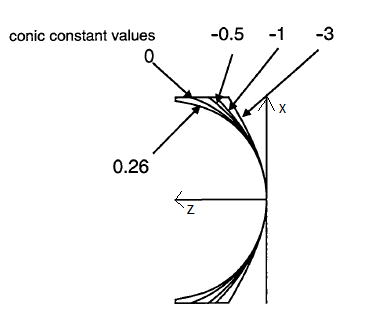
\includegraphics[width=.4\textwidth]{Immagini/Chapter2/SurfaceConic1}
%
\caption{Different kind of surface conic, with the same $c $ curvature value, and different constant $k $.}
%
\label{fig: SurfaceConic1}
%
\end{figure}
\noindent A good point that have the conical surfaces is the possible elimination of spherical aberration. As said in before, the spherical surface is affected by spherical aberration if the configuration is away from the normal incidence. The ellipsoidal geometry forms a point-to-point free-aberration focus where source and image are both real. On the contrary the hyperbola work for conjugates foci on different side of it. A parabolic surface creates a perfect image for any axial object place at infinity, this is the reason why parabolic mirror are very used for astronomical application. For all the shapes of surfaces, if the object is moved from its ideal position aberration will appear: an axial movement introduce a certain amount of spherical aberration, lateral movement introduce other types of aberration such as coma, astigmatism and field curvature.
\\
\noindent 
Figure \ref{fig :spher abb corr} show a simple example of how it is possible to correct the spherical aberration using a paraboloid mirror \ref{fig: ParabolicMirror} instead of a spherical mirror \ref{fig: Sphericalmirror}
\begin{figure}[]
%
\centering
%
\subfloat[][Spherical mirror \label{fig: Sphericalmirror}]
   {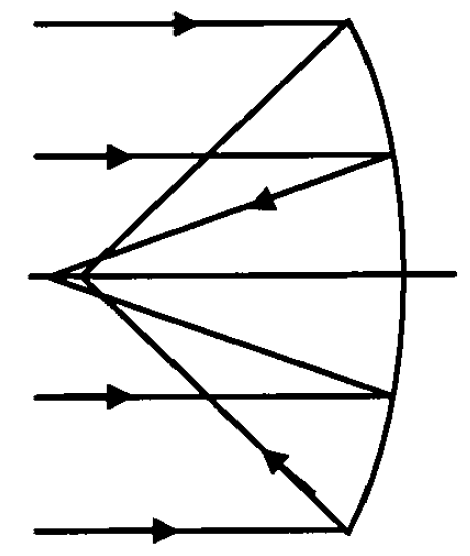
\includegraphics[width=.2\textwidth]{Immagini/Chapter2/SphericalMirror}}\quad
%
\subfloat[][Parabolic Mirror  \label{fig: ParabolicMirror}]
   {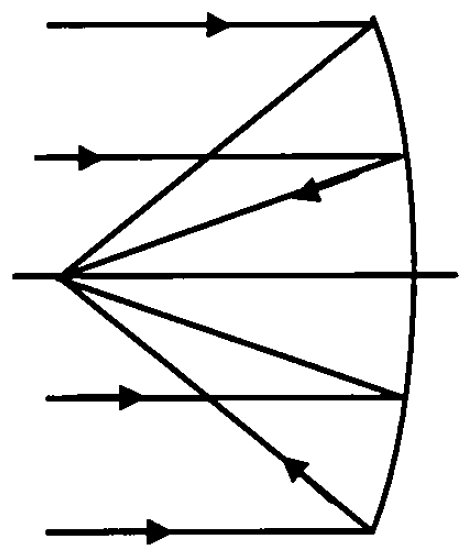
\includegraphics[width=.2\textwidth]{Immagini/Chapter2/ParabolicMirror}}
%
\caption{Example of spherical aberration correction}
\label{fig :spher abb corr}
%
\end{figure}

\section{Compound Optical system}
Simple mirror work well for a point-to-point optical system, but, to reproduce correctly an object image with the same aspect ratio it needed an imaging system. A system like this must satisfy the Sine-Abbe condition
\begin{equation}
\frac{sin u^{'}}{sin U^{'}} = \frac{sin u}{ sin U}
\label{eq: SineAbbe}
\end{equation} 
\noindent where, as it is showed in Figure \ref{fig: SineAbbe}, $u $ and $u^{'} $ are rays that leave the object, $U$ and $U^{'} $ are the angles of the same rays that reach the image plane. In other words, the sine of the ray that leave the object must be proportional to the sine of the angles that reach the image plane.
\begin{figure}[]
%
\centering
%
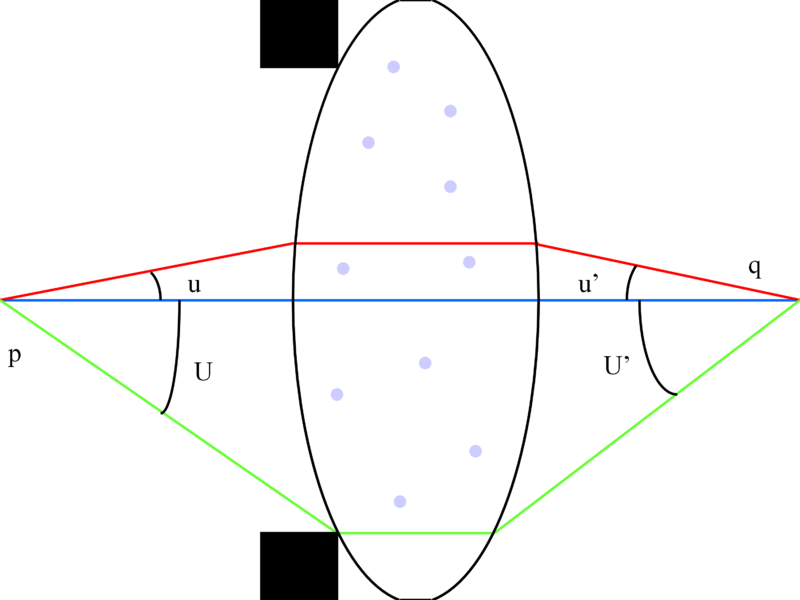
\includegraphics[width=.6\textwidth]{Immagini/Chapter2/SineAbbeCondition}
%
\caption{Sine Abbe condition for a lens}
%
\label{fig: SineAbbe}
%
\end{figure}
Unfortunately, for the case of mirror, there is no way to satisfy the Sine Abbe condition using only one mirror. To satisfy the condition, and so obtain a better image, there are optical systems composed by more than one mirror. One is the Wolter system, widely used in astronomy, that use a combination of coaxial and confocal conic section. A first approximation system that respects the sine Abbe condition are the Kirkpatrick-Baez and Montel system. These systems are compound optical systems involving meridian focusing at right angle planes.
\subsection{Wolter System} 
\hspace{10mm} In 1952 Wolter published a paper \cite{wolter1975mirror} in which he discussed several dispositions of two conical mirrors in order to collect light for an astronomical use. Figure \ref{fig: Wolter I/II/III} show the different type op systems: Wolter $\mathrm{I} $, Wolter $\mathrm{II} $, Wolter $\mathrm{III} $.\noindent
Wolter $\mathrm{I} $ telescope consist of a coaxial paraboloid (primary mirror) and hyperboloid (secondary mirror). The focus of the paraboloid is coincident with the rear focus of the hyperboloid, and the reflection inside both mirrors. The Wolter $\mathrm{II} $ telescope use the same kind of mirror of Wolter $\mathrm{I} $ paraboloid and hyperboloid. But the focus of the paraboloid coincident with the front focus of the hyperboloid, and, the reflection, occurs internally for the paraboloid and externally for the hyperboloid. The Wolter $\mathrm{III} $ telescope consist in a paraboloid and an ellipse. In this system the first mirror is the paraboloid one, and the second is the ellipsoidal that have front focus coincident with that of the parabola, moreover the reflection is external for the paraboloid and internal for the ellipsoidal.
\noindent The Wolter $\mathrm{I} $ have typical grazing angle of less than a degree and is used for hard X-rays. The Wolter $\mathrm{II} $ telescope has typical grazing angle of, approximate, 10 degree and is used for soft X rays and extreme ultraviolet (EUV).
\noindent Because of circular symmetry, astigmatism and spherical aberration are eliminated but  exhibit coma aberration. Other problem is the difficulty of fabrication , and require a huge area to achieve a very small collecting angle.
\begin{figure}[]
%
\centering
%
\subfloat[][Wolter I  \label{fig: Wolter1}]
   {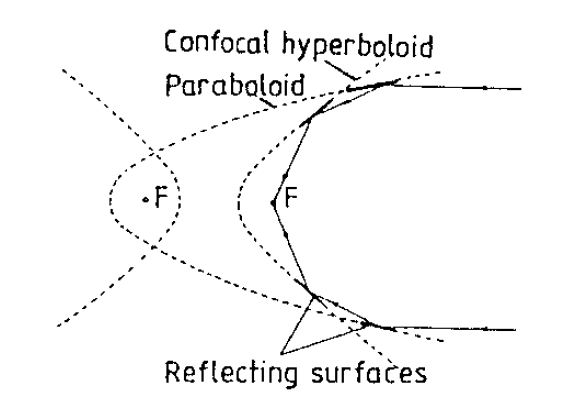
\includegraphics[width=.4\textwidth]{Immagini/Chapter2/Wolter1}}
%
\subfloat[][Wolter II \label{fig: Wolter2}]
   {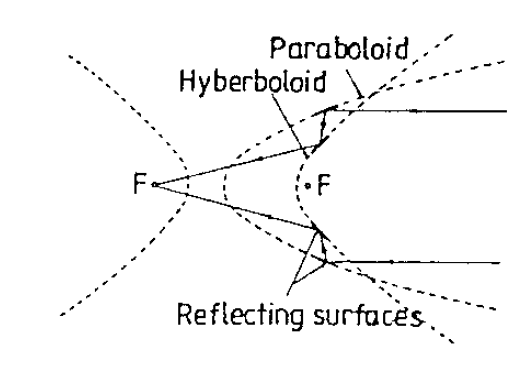
\includegraphics[width=.4\textwidth]{Immagini/Chapter2/Wolter2}}\quad
%
\subfloat[][Wolter III  \label{fig: Wolter3}]
   {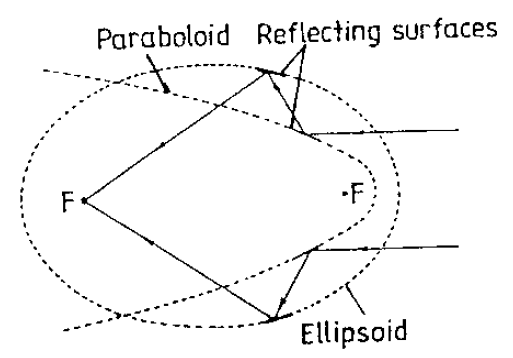
\includegraphics[width=.4\textwidth]{Immagini/Chapter2/Wolter3}}
%
\label{fig :Wolter Systems}
%
\caption{Different kind of Wolter System \cite{X-RayWolter}}
%
\label{fig: Wolter I/II/III}
%
\end{figure}

\subsection{Kirkpatrick-Baez System }

\hspace{10mm} In 1948, Kirkpatrick and Baez proposed (\cite{kirkpatrick1948formation}) an X-ray focusing optical system consisting of two total reflection elliptical mirrors, which aligned perpendicularly (Figure \ref{fig: KirckPatrick Baez System}). This focusing optical system is very popular at the ESRF due to its potential to remarkably improve the performance characteristics of X-ray by enabling more efficient collecting of X-rays than in other methods. A further advantage is that the method maintains the focusing state with the same optical arrangement even if the wavelength of the X-rays is shifted. However, to realize X-ray beams with an ideal focal size, high efficiency and absence of background noise around a main peak, it is necessary to prepare elliptical mirrors having a very high quality. Since the two mirrors are not coincident, the object distance for the meridian reflection in the first mirror is less than that for the sagittal reflection in the second mirror. Thus, the magnification is different in the two directions.
\begin{figure}[H]
%
\centering
%
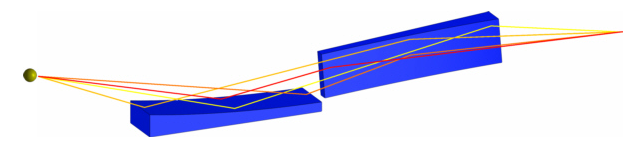
\includegraphics[width=.6\textwidth]{Immagini/Chapter2/KBSystem}
%
\caption{Kirkpatrick-Baez system}
%
\label{fig: KirckPatrick Baez System}
%
\end{figure}


\section{Montel}
Another possibility to dispose mirrors creating a focalizing or colimating optical system consist in the disposition of two orthogonal mirrors attached one to the other as showed in Figure \ref{fig: MontelSystem1}. This geometry is called Nested Kirkpatrick-Baez system or Montel system \cite{montel1957x}. To go beyond current state-of-art performances, new approaches are required that can collect more divergence than with standard sequential Kirkpatrick-Baez (KB) X-ray mirrors. Indeed, the quality of x-ray mirrors has now reached the diffraction limit, and simply more perfect KB mirrors cannot decrease spot size because of different magnification in horizontal and vertical.
\\
In this section we first describe of the Montel system with its advantages and disadvantages with respect to the KB system. Then there is an explanation on the optical design method.

\subsection{Description}
\hspace{10mm} Because of its distinctive design, Montel system have numerous advantages over traditional Kirkpatrick–Baez system. In contrast to KB systems where the two reflective surfaces are arranged in-line one after the other, those in Montel optics are mounted side by side at 90 to each other (Figure \ref{fig: MontelSystem1}). Due to this fact, the incident X-ray beam now undergoes reflection simultaneously from both surfaces instead of being reflected sequentially as in the KB system. Hence, the mirror-focal point distance is diminished and consequently the demagnification ratio increased. The gain can be substantial especially when the focal distance is comparable with the mirror lengths. Furthermore, the side-by-side geometry offers a more compact design and therefore represents a convenient solution when space availabilities for optical elements are highly restrictive. In terms of mechanical structures, KB optics usually require two independent sets of alignment stages for each mirror. It is possible, in the Montel system, to assemble both surfaces together with their stages onto a common platform. Apart from providing a compact solution, this can also help in reducing the sources of parasitic vibrations as well as any individual misalignment between the mirrors. Lastly, since in this geometry that want to the second mirror is positioned closer to the source than in the KB system, for the same angular acceptance in both mirror systems, a shorter mirror is needed in the Montel optics design. This is highly desirable as significantly better figure errors can be achieved for smaller mirror sizes than larger ones with the overall benefit of yielding less aberrated beams.
\begin{figure}[H]
%
\centering
%
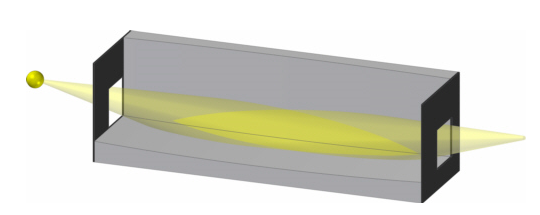
\includegraphics[width=.6\textwidth]{Immagini/Chapter2/MontelSystem}
%
\caption{Montel system}
%
\label{fig: MontelSystem1}
%
\end{figure}
%
\noindent However Montel configuration, presents some draw-back with respect to the sequential KB system. The fact that the beam hit the worst part of the mirrors, the edge, that are less polished thus contain more surface defect, decreases the quality of the reflection.
\subsection{Optical Design \cite{ice2009nested}}
The mirrors used in this Montel configuration are mirror that have a plane shape in one direction and elliptical shape in the other direction. They are cylinders of elliptical section. One approach to obtain the Montel system is that to use two pre-figured elliptical mirrors and grind the cut side at 45$^\circ $ as shown in Figure \ref{MontelEdges}. Then the mirrors are placed together making a good fit with no gap requiring no contouring of the mirror side. Another way involves dividing pre-figured elliptical mirror into two parts that are added  together, forming the Montel system. These approaches are primary driven by the fact that in a conventionally polished mirror the clear aperture area has the best figure and finish. As such, using two halves of a prefigured mirror cut in the middle has several advantages- including consistency and economy. There are major challenges however. First, the mirror surface must be protected against damage and deformation during cutting and subsequent figuring operations. After cutting into two, the cut sites must be treated (e.g., etched) to remove any subsurface damages that could alter a mirror's figure. Then the mating side of one of the mirrors must be contoured and polished such that when it is placed against the partner mirror, it makes a nearly perfect fit with good surface quality all the way to the contact edge This last two-steps are crucial because if there is a significant gap or if the mirror surfaces in the vicinity of the interface are damaged, a significant part of the incident beam could be lost. As an example, are developed a pair of Montel mirrors for poly-chromatic nano focusing on Sector 33 at APS. This beam line will use 40 mm long elliptical mirrors for nano-focusing a 100 $\mu m$ beam to a 50 nm spot at 2000x demagnification. This concave elliptical mirror has a maximum depression of about 6 $\mu m$ at its centre. If cut flat and placed against its mating mirror, a gap as large as 6 $\mu m$ is created which loses about 10$\% $ of the 100 $\mu m$ incident beam. Similarly, if the mirror surfaces near the intersection are damaged, then beam loss can be significant.
\begin{figure}[]
%
\centering
%
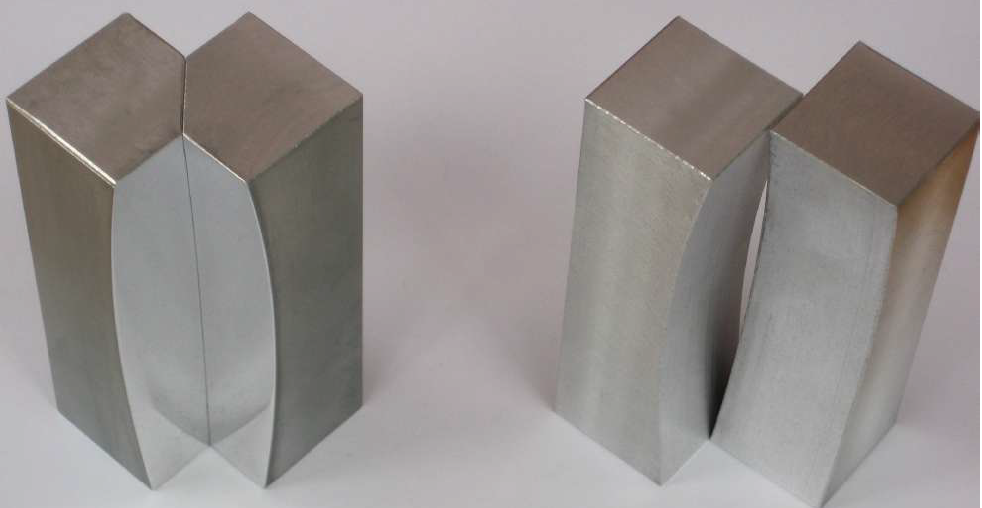
\includegraphics[width=.8\textwidth]{Immagini/Chapter2/MontelEdges}
%
\caption{Example of how a Montel system is built from two cylindrical mirrors cutting the edge with at angle of $45^{\circ} $.}
%
\label{fig: MontelEdges}
%
\end{figure}
